\chapter{Appendices}

\section{Appendix 1}

API Documentation:

\begin{center}
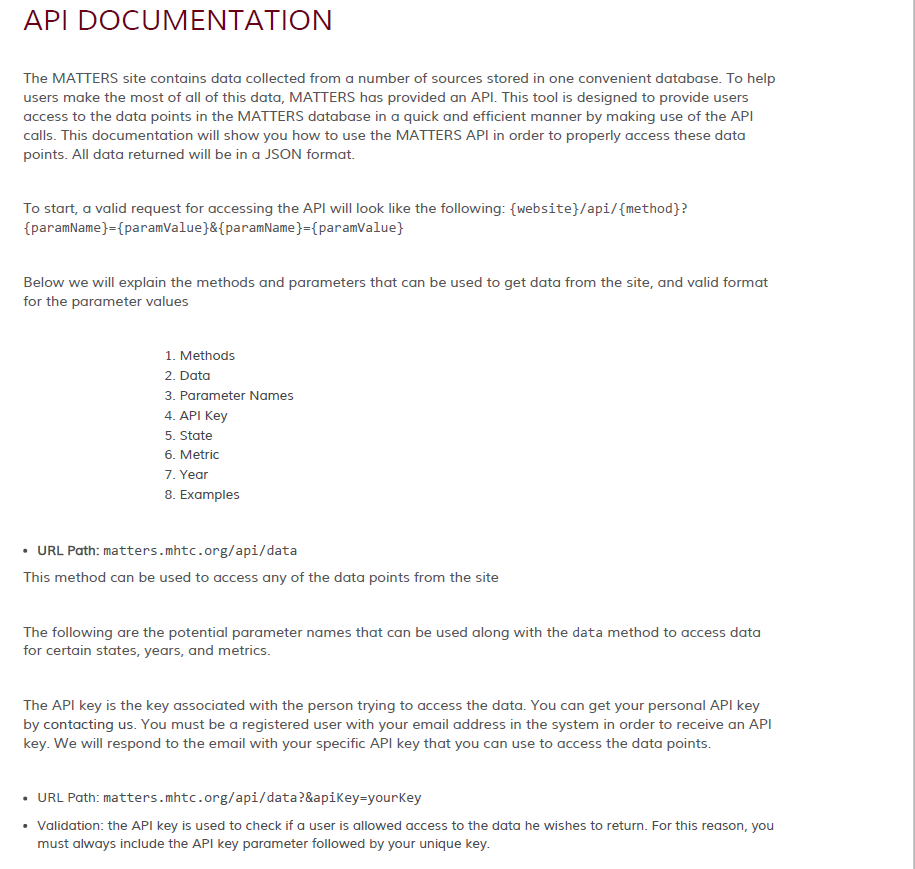
\includegraphics[width=0.9\linewidth]{images/docs1}
\end{center}

\begin{center}
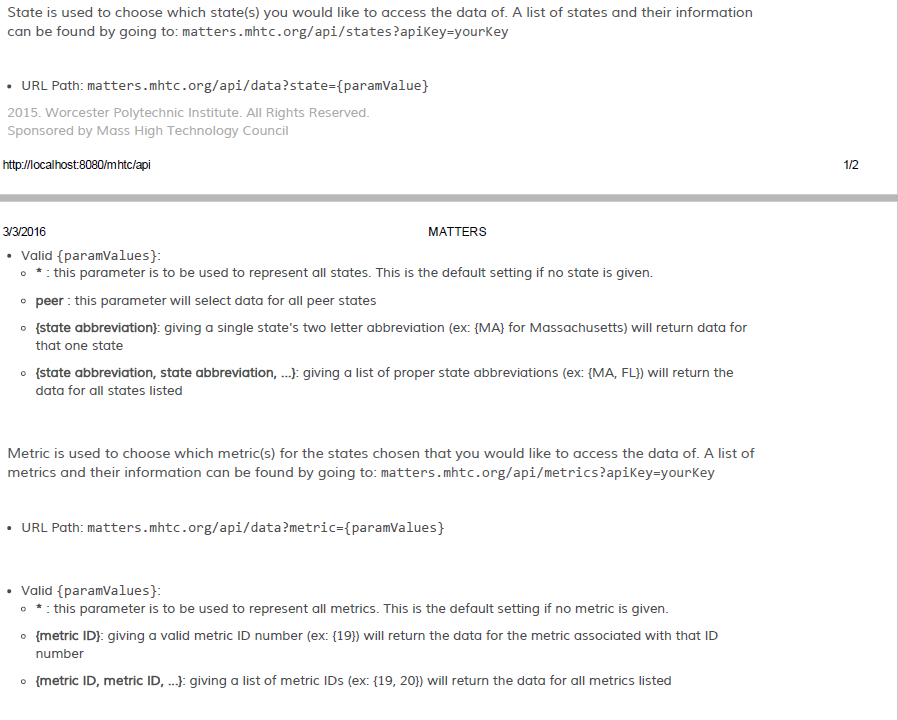
\includegraphics[width=0.9\linewidth]{images/docs2}
\end{center}

\begin{center}
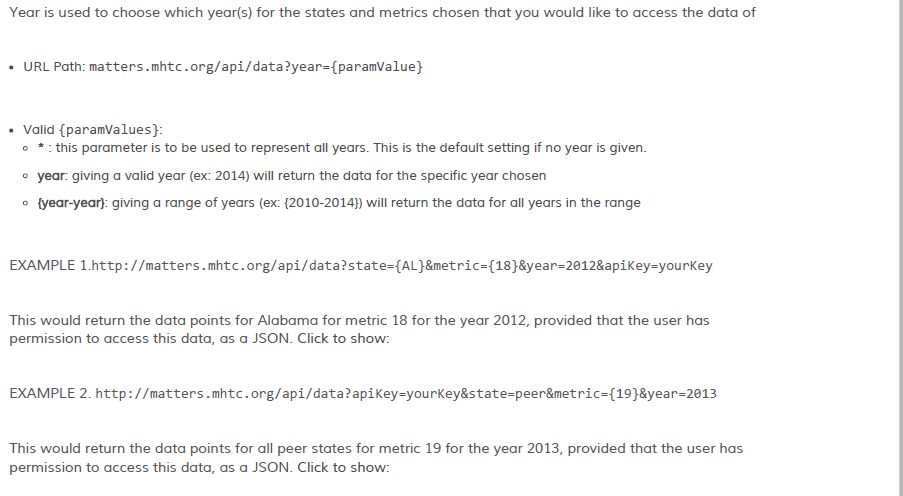
\includegraphics[width=0.9\linewidth]{images/docs3}
\end{center}

\section{Appendix 2}

Full User Study documents.

\subsection{Informed Consent Agreement for Participation in a Research Study}

Investigator: Jillian Hennessy or Dmytro Bogatov 

Contact Information: Jillian (jrhennessy@wpi.edu) or Dmytro (dbogatov@wpi.edu)

Title of Research Study: Metric Builder and API Documentation User Testing


Introduction 
You are being asked to participate in a research study.  Before you agree, however, you must be fully informed about the purpose of the study, 
the procedures to be followed, and any benefits, risks or discomfort that you may experience as a result of your participation.  
This form presents information about the study so that you may make a fully informed decision regarding your participation. 

Purpose of the study:  The purpose of this study is to test and receive user feedback on our Metric Builder and API features of the MATTERS site. 
We are looking to see how easy it is use these features and if there are any changes to the design that need to be made.

Procedures to be followed:  You will be asked to use the Metric Builder and API and complete a set of tasks given to you. 
During this time, you will be observed by the instructor to see how you navigate the site/ how long these tasks take to complete. 
After completing the tasks, you will be given a short survey about your experience with the Metric Builder and API features and their design.

Risks to study participants:  There are no risks to you if you choose to take part in this user study. 
You may choose to stop this study at any time and your responses/ observation will not be used. 

Benefits to research participants and others:  There are no direct benefits to completing this study. You will be helping our MQP 
team to ensure our features are ready to be deployed and used by their intended targets as well as find any potential problems 
with the features that we may want to fix.

Record keeping and confidentiality: We will not use any of your personal information as part of the results of the study. 
Our observations will be linked to the ID of the survey however your name will not be used. Any responses given in the survey will remain anonymous. 
Records of your participation in this study will be held confidential so far as permitted by law. However, the study investigators, 
the sponsor or it's designee and, under certain circumstances, the Worcester Polytechnic Institute Institutional Review Board 
(WPI IRB) will be able to inspect and have access to confidential data that identify you by name.  
Any publication or presentation of the data will not identify you.

Compensation or treatment in the event of injury:  You do not give up any of your legal rights by signing this statement.

For more information about this research or about the rights of research participants, or in case of research-related injury, contact: 
Please see the contact information at the beginning of this document. In addition, you may also contact the IRB Chair 
(Professor Kent Rissmiller, Tel. 508-831-5019, Email:  kjr@wpi.edu) and the University Compliance Officer (Jon Bartelson, Tel. 508-831-5725, Email:  jonb@wpi.edu).

Your participation in this research is voluntary.  Your refusal to participate will not result in any penalty to you or any loss of benefits to 
which you may otherwise be entitled.  You may decide to stop participating in the research at any time without penalty or loss of other benefits.  
The project investigators retain the right to cancel or postpone the experimental procedures at any time they see fit. 

By signing below, you acknowledge that you have been informed about and consent to be a participant in the study described above.  
Make sure that your questions are answered to your satisfaction before signing.  You are entitled to retain a copy of this consent agreement.

\subsection{Script for Investigators}

*Have them look over and sign the consent form*

*You will also sign the consent form*

*Have them complete part one of the survey*

User Study Tasks: Part 1, Metric Builder feature

*log them into the MATTERS site so they have access to the Metric Builder feature*

*we will observe as they complete the tasks, and will record the time for how long it takes to find the metric builder page, and their metric in the data explorer*

*if they cannot find the link in a reasonable time, bring them to the Metric Builder page and make a note*

Navigate to the “Metric Builder” feature
Please create your own metric formula, which includes Unemployment Rate, Corporate Income Tax Rate and Median Household Income, with weights 10, 5, and 22 respectively.

Name your new metric “My Metric” and save it.

Please find and select your created metric on the “data explorer” page.

Edit your metric formula so that Unemployment Rate is no longer a part of the metric and Median Household Income  has a weight of 15.

Save your changes to “My Metric”.

Please delete “My Metric”

You will now receive a short survey about your experience using the Metric Builder.

*Have them complete part 2 of the survey on their own*

User Study Tasks: Part 2, API feature and Documentation

*we will observe as they complete the tasks, and will record the time for how long it takes to find the API Docs page*

*if they cannot find the link in a reasonable time, bring them to the API Docs page and make a note*

Navigate to the API Documentation page

Your API Key is “secret”

Please get the data for the metric Unemployment Rate for Massachusetts and Florida for the year 2012 using the API tool and the documentation as a guide

You will now receive a short survey to complete about your experience using the API and API Documentation.

*Have them complete part three of the survey*

*Upon completion make sure the survey has been submitted, ask them if they have any other questions or feedback, make any notes, and thank them for participating*

\subsection{Survey}

\begin{center}
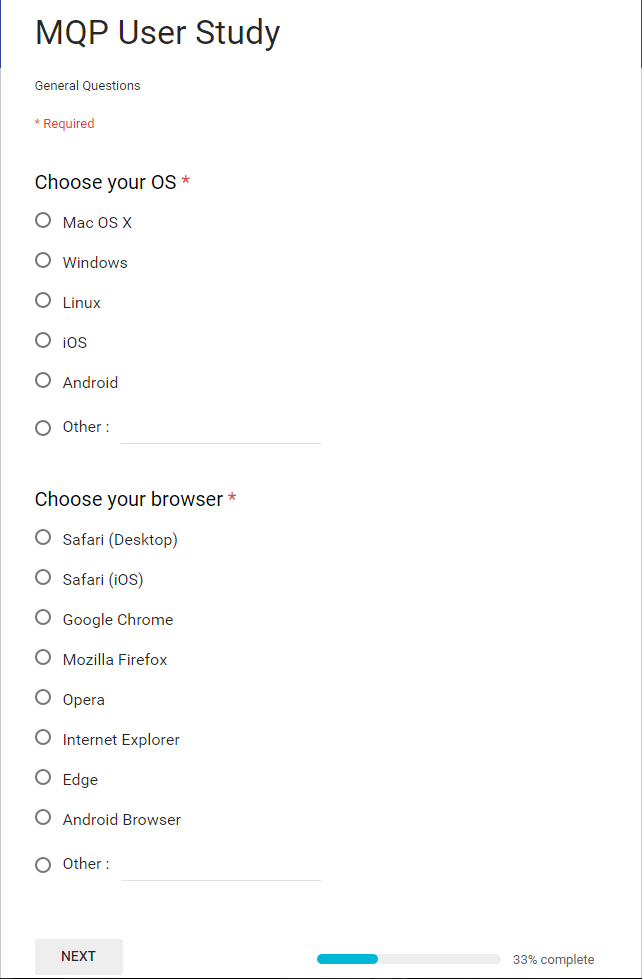
\includegraphics[width=0.9\linewidth]{images/survey1}
\end{center}

\begin{center}
	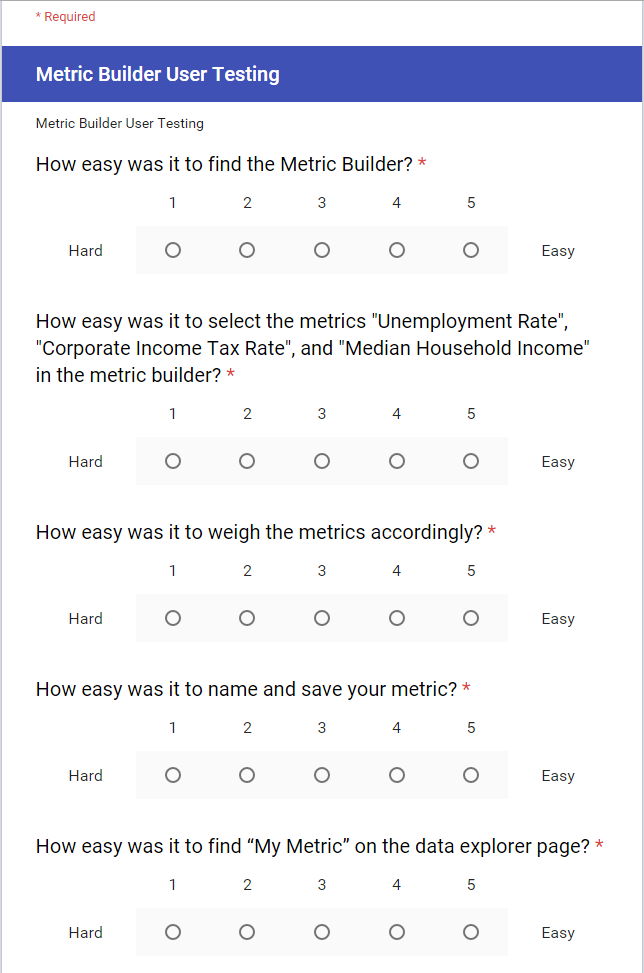
\includegraphics[width=0.9\linewidth]{images/survey2}
\end{center}

\begin{center}
	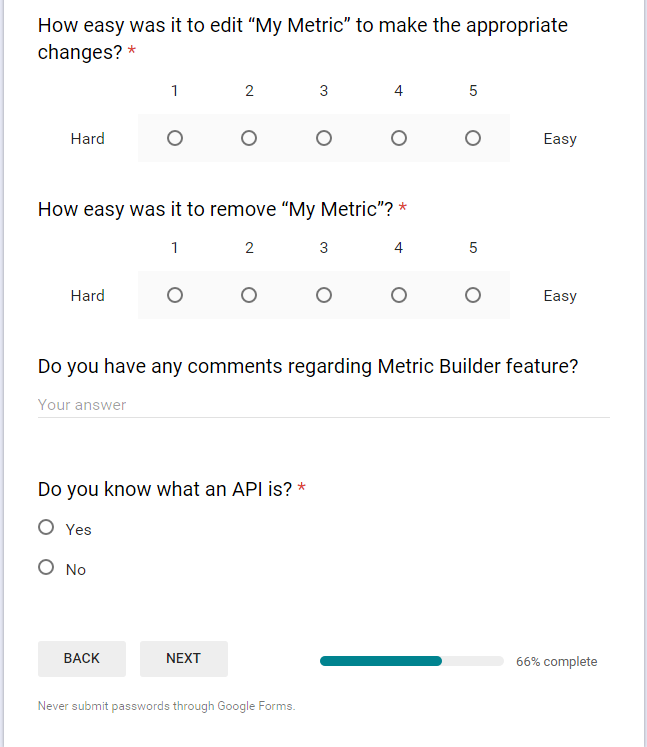
\includegraphics[width=0.9\linewidth]{images/survey3}
\end{center}

\begin{center}
	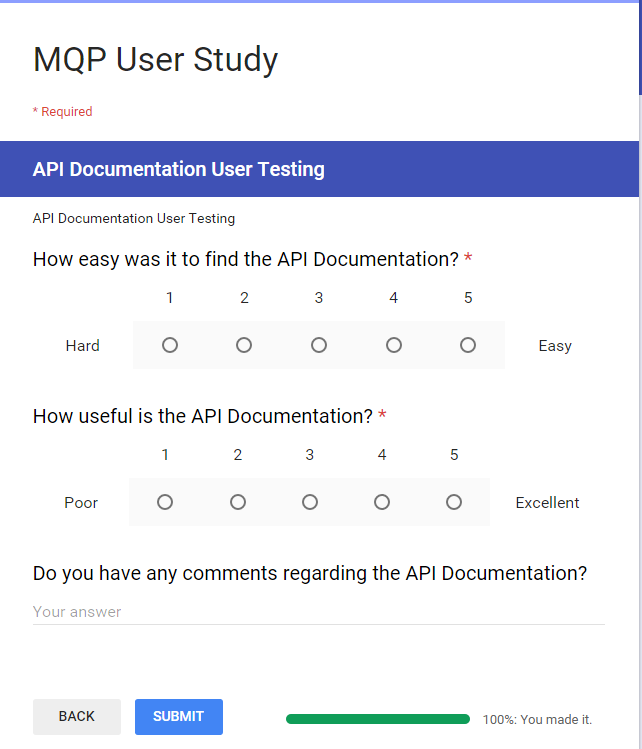
\includegraphics[width=0.9\linewidth]{images/survey4}
\end{center}

\subsection{Results}

Full user survey results and comments can be found in the Excel file labeled User Results